\documentclass[tikz,border=6pt]{standalone}
\usepackage{amsmath,amssymb,mathtools,physics,bm,nicefrac,wasysym}
\usepackage{xcolor}

\definecolor{colone}{RGB}{180,60,60}
\definecolor{coltwo}{RGB}{60,110,180}
\definecolor{colthree}{RGB}{60,140,80}

\definecolor{accent}{HTML}{A13D2C}
\definecolor{accent2}{HTML}{2B5F6B}
\definecolor{muted}{HTML}{5A564F}
\definecolor{panel}{HTML}{F8F6F0}
\definecolor{linecol}{HTML}{D8D2C4}
\definecolor{ink}{HTML}{1E1C1A}
\definecolor{astroblue}{HTML}{1B4F72}
\definecolor{astrodark}{HTML}{17202A}
\definecolor{sunyellow}{HTML}{E8A33D}

\usetikzlibrary{calc,arrows.meta,positioning,decorations.pathreplacing,decorations.markings,angles,quotes,shapes.geometric}
\usepackage{tikz-3dplot}

\newcommand{\vecr}{\vec r}
\newcommand{\vecL}{\vec L}
\newcommand{\vecA}{\vec A}
\newcommand{\vecf}{\vec f}
\newcommand{\vecF}{\vec F}
\newcommand{\vecp}{\vec p}
\newcommand{\avg}[1]{\left\langle #1\right\rangle}
\newcommand{\vecx}{\vec x}
\newcommand{\hatn}{\hat n}
\newcommand{\rhat}{\hat r}
\newcommand{\phihat}{\hat\phi}
\newcommand{\thetahat}{\hat\theta}
\newcommand{\note}[1]{\textcolor{blue!60!black}{\textit{[#1]}}}

\newcommand{\LST}{\mathrm{LST}}
\newcommand{\GST}{\mathrm{GST}}
\newcommand{\GMST}{\mathrm{GMST}}
\newcommand{\GAST}{\mathrm{GAST}}
\newcommand{\LMST}{\mathrm{LMST}}
\newcommand{\LAST}{\mathrm{LAST}}
\newcommand{\UT}{\mathrm{UT}}
\newcommand{\UTC}{\mathrm{UTC}}
\newcommand{\TAI}{\mathrm{TAI}}
\newcommand{\TT}{\mathrm{TT}}
\newcommand{\TDB}{\mathrm{TDB}}
\newcommand{\JD}{\mathrm{JD}}
\newcommand{\MJD}{\mathrm{MJD}}
\newcommand{\EoT}{\mathrm{EoT}}
\newcommand{\SNR}{\mathrm{SNR}}
\newcommand{\RON}{\mathrm{RON}}



\begin{document}
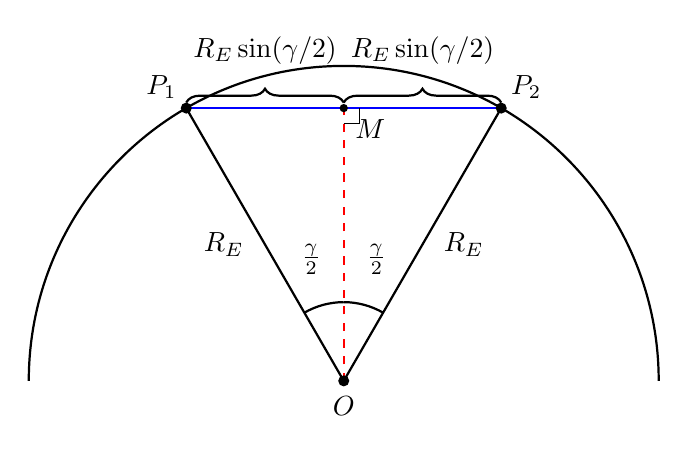
\begin{tikzpicture}
    % Define the radius and angle
    \def\RE{4}
    \def\gammaangle{60}

    % Define coordinates rotated by 90 degrees
    \coordinate (O) at (0,0);
    \coordinate (A) at (90+\gammaangle/2:\RE);
    \coordinate (B) at (90-\gammaangle/2:\RE);
    
    % M is the midpoint of the chord for the perpendicular bisector
    \coordinate (M) at (90:{\RE*cos(\gammaangle/2)});

    % Draw the circle background and top arc
    %\draw[dashed, gray!70] (O) circle (\RE);
    \draw[thick] (0:\RE) arc (0:180:\RE);

    % Draw the radii
    \draw[thick] (O) -- (A) node[midway, left=4pt] {$R_E$};
    \draw[thick] (O) -- (B) node[midway, right=4pt] {$R_E$};

    % Draw the full chord
    \draw[thick, blue] (A) -- (B);

    % Draw the perpendicular bisector
    \draw[thick, dashed, red] (O) -- (M);

    % Right angle marker at the intersection
    \draw (M) ++(0,-0.2) -- ++(0.2,0) -- ++(0,0.2);

    % Label the half-chord distances using braces
    \draw[decorate, decoration={brace, amplitude=5pt, raise=2pt}, thick]
         (A) -- (M) node[midway, above=12pt] {$R_E \sin(\gamma/2)$};
    \draw[decorate, decoration={brace, amplitude=5pt, raise=2pt}, thick]
         (M) -- (B) node[midway, above=12pt] {$R_E \sin(\gamma/2)$};

    % Draw and label the split angles
    \pic [draw, thick, "$\frac{\gamma}{2}$", angle eccentricity=1.6, angle radius=1cm] {angle = M--O--A};
    \pic [draw, thick, "$\frac{\gamma}{2}$", angle eccentricity=1.6, angle radius=1cm] {angle = B--O--M};

    % Mark and label the points
    \fill (O) circle (2pt) node[below=2pt] {$O$};
    \fill (A) circle (2pt) node[above left] {$P_1$};
    \fill (B) circle (2pt) node[above right] {$P_2$};
    \fill (M) circle (1.5pt) node[below right=1pt] {$M$};
\end{tikzpicture}
\end{document}
